\subsection{Introduction}
	\begin{figure}[h]
		\centering
		\begin{subfigure}{0.49\linewidth}
			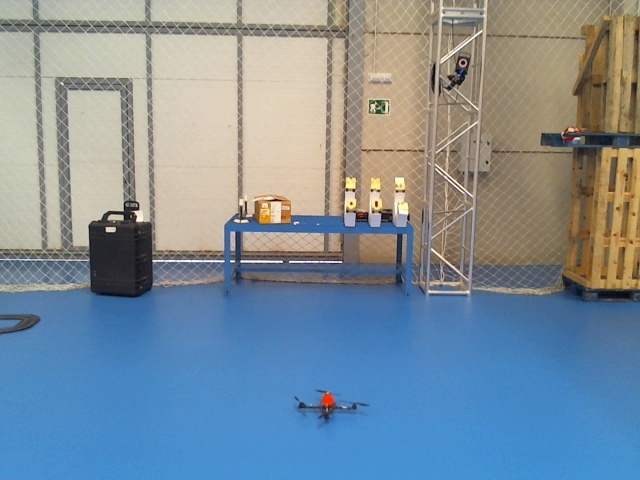
\includegraphics[width=\linewidth]{../Images/c4/image_ori}
			\caption{Original Image}
			\label{fig:image_ori}
		\end{subfigure}
		%--------------------------------------------------------------------
		\begin{subfigure}{0.49\linewidth}
			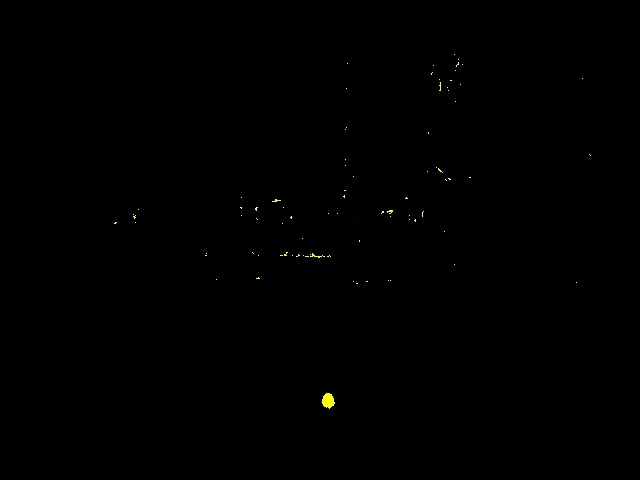
\includegraphics[width=\linewidth]{../Images/c4/image_seg}
			\caption{Segmented Image}
			\label{fig:image_seg}
		\end{subfigure}
		\caption{Images to and from algorithm}
		\label{fig:frames_PC}
	\end{figure}

	La figura: \ref{fig:frames_PC} muestra una imagen del dataset capturada por las c\'amaras de los quadqrotors y el resultado de la segmentaci\'on por color. Sin embargo, a diferencia de las simulaciones en esta hay m\'ultiples objetos pequeños que tienen que ser cribados con un filtro de color y de tama\~no.

\subsection{Simulaci\'on no distribuida}	
	\subsubsection{Algoritmo de seguimiento terrestre}
	
	Los datasets fueron grabados en est\'ereo. Sin embargo, las primeras pruebas fueron con los objetivos en tierra por lo que usando la informaci\'ion de una sola de las c\'amaras puede probarse el algoritmo. La siguiente tabla muestra unos estad\'isticos del algoritmo: \\
	
	{
	\centering
		\begin{tabular}{|c|c|c|c|c||c|}
		\hline  					&  Open Image	&  RGB to HSV 	& Segmentation 	& EKF step  & Complete \\ 
		\hline  \textbf{time (ms)}	& 0.0085 		& 0.0015 		& 0.0100 		& 0.0001 	& 0.0231 	\\ 
		\hline  \textbf{fps (1/s)}	&  118			&  645			&  100			& 13936 	& 43 		\\ 
		\hline 
		\end{tabular} 
	}
	\newline

	{
	\label{Reference_fps_table}
	En este caso se hizo una prueba del algoritmo ejecut\'andose de forma secuencial por lo que puede aumentarse la velocidad del mismo paralelizando los procesos en diferentes threads. En la siguiente secci\'on se mostrar\'an los resultados dentro de los ordenadores de abordo con el algoritmo en paralelo. \ref{test_with_odroid_and_GT}
	}
	
	Las siguientes gr\'aficas muestran los resultados de las trayectorias \ref{fig:trajectories_PC} y los errores de estimaci\'on   \ref{fig:errors_PC}. Los errores est\'an acotados superiormente por $0.2 m$.
	\begin{figure}
	     \centering
	     \begin{subfigure}[b]{0.4\textwidth}
			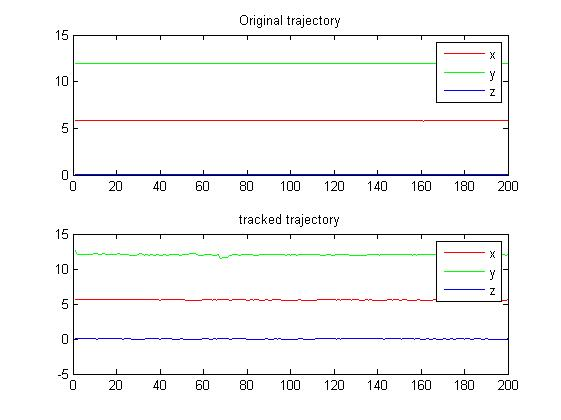
\includegraphics[width=\linewidth]{../Images/c4/trajs}
			\caption{Ejecuci\'on no distribuida  - Trayectorias original y Calculadas.}
			\label{fig:trajectories_PC} 
	     \end{subfigure}%
	     ~
	     \begin{subfigure}[b]{0.4\textwidth}
			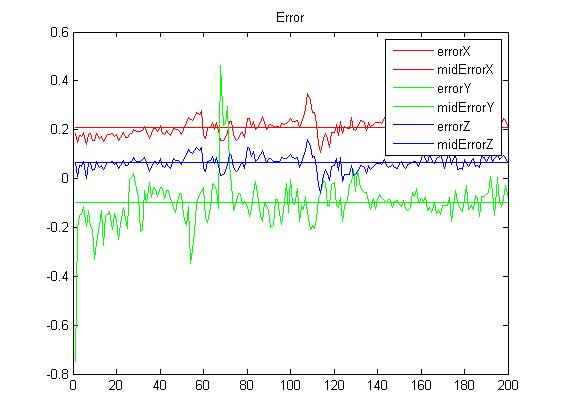
\includegraphics[width=\linewidth]{../Images/c4/errors}
			\caption{Ejecuci\'on no distribuida - Errores}
			\label{fig:errors_PC}
	     \end{subfigure}
	     \caption{$Head Scene$}
	\end{figure}

	
	\newpage
	
	%\begin{figure}[ht]
	%	\centering
	%	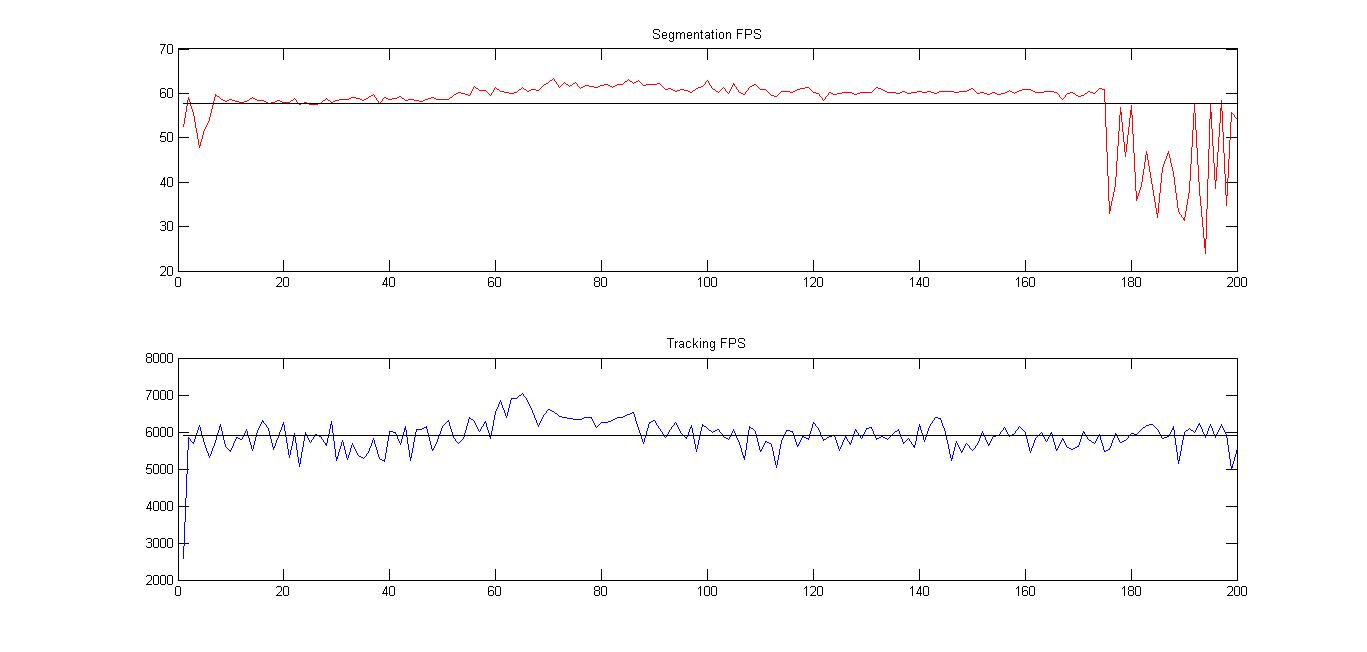
\includegraphics[width=\linewidth]{../Images/c4/fps}
	%	\caption{}
	%	\label{fig:fps_PC}
	%\end{figure}
		
	\subsubsection{Algoritmo de seguimiento est\'ereo}
	
	En este caso se usa la informaci\'on de ambas c\'amaras para la estimaci\'on de posici\'on: \\
		
	{                
	\centering
		\begin{tabular}{|c|c|c|c|c||c|}
		\hline  					&  Open Image	&  RGB to HSV 	& Segmentation 	& EKF step  & Complete \\ 
		\hline  \textbf{time (ms)}	&	0.0222		& 	0.0031 		&  	0.0157		&  	0.0001 	&  0.0429		\\ 
		\hline  \textbf{fps (1/s)}	& 	45 			& 	321.5 		& 	63.8 		& 9785.5	&  23.3		\\ 
		\hline 
		\end{tabular} 
	}
	\newline
	
	Esta tabla tiene la misma notaci\'on que la tabla anterior \ref{Reference_fps_table}.
	
	Final mente estas im\'agenes muestran las posiciones originales y calculadas del objetivo \ref{fig:trajectories_stereo_PC} y el error entre ellas \ref{fig:errors_stereo_PC}.
	
	\begin{figure}[hp]
		\centering
		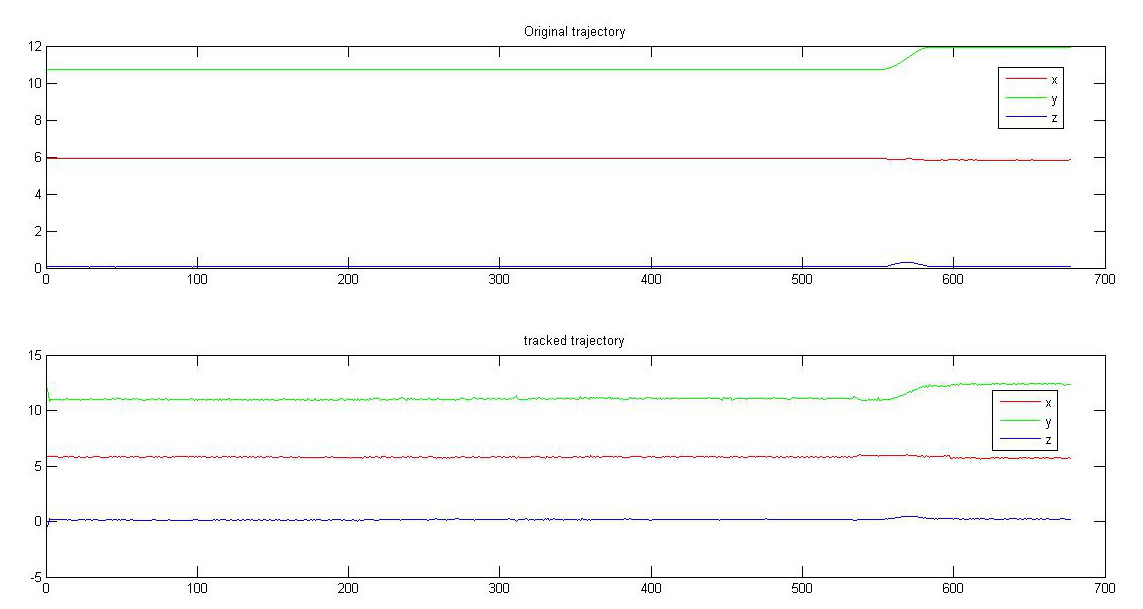
\includegraphics[width=\linewidth]{../Images/c4/trajs_stereo}
		\caption{Algoritmo de seguimiento est\'ereo - Trayectorias original y calculada}
		\label{fig:trajectories_stereo_PC}
	\end{figure}
	
	\begin{figure}[htp]
		\centering
		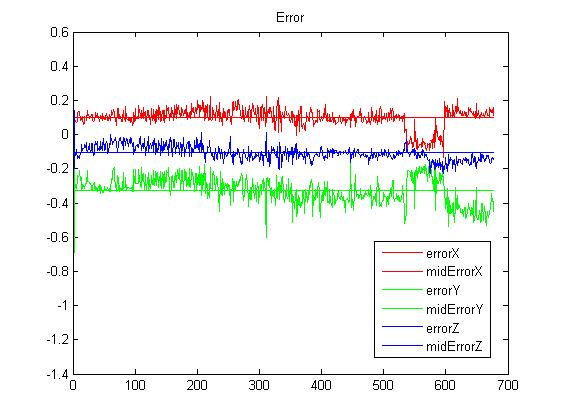
\includegraphics[width=0.7\linewidth]{../Images/c4/errors_stereo}
		\caption{Algoritmo de seguimiento est\'ereo - Errores}
		\label{fig:errors_stereo_PC}
	\end{figure}	
	

\newpage	
\subsection{Experimento distribuido}
	\label{test_with_odroid_and_GT}
	
	\begin{wrapfigure}{r}{0.5\linewidth}
		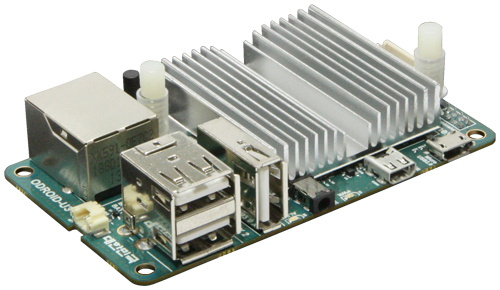
\includegraphics[width=\linewidth]{../Images/c4/odroidu3}
		\caption{Hardkernel Odroid u3}
		\label{fig:odroidu3}
	\end{wrapfigure}
		
	Para estos test se us\'o el esquema de software descrito en secciones anteriores para la estaci\'on en tierra \ref{fig:GroundStation} y para el quadrotor \ref{fig:Quadsoftware}, conectados a trav\'es de la red. 
	
	\subsubsection{Algoritmo de seguimiento terrestre}
	
	La siguiente tabla muestra los tiempos de ejecuci\'on de cada ciclo de cada hilo del quadrotor:
	% 666 TODO: quitar el filtro de media del tratamiento que ralentiza mucho
	\newline
	\newline
	{
	\centering
		\begin{tabular}{|c|c|c|c|c|c|}
		\hline  					&  Open Img	&  cp Img 	& Vicon 	& Treat img & Comm  		\\ 
		\hline  \textbf{time (ms)}	& 	0.0154	& 0.0018	&	0.00096	&  	 0.019	&	0.0001		\\ 
		\hline  \textbf{fps (1/s)}	&  	68		&  63.2		&  10356	&  	51.23	&	12022		\\ 
		\hline 
		\end{tabular} 
	}
	\newline
	
	Y esta segunda tabla de la estaci\'on en tierra:
	\newline
	
	{
	\centering
		\begin{tabular}{|c|c|c|}
		\hline  					&  comm		&  EKF step	\\
		\hline  \textbf{time (ms)}	& 	0.0001	& 	0.0001	\\
		\hline  \textbf{fps (1/s)}	&  	10567.5	&  	9608.5	\\
		\hline 
		\end{tabular} 
	}
	\newline
	
	El cuello de botella se encuentra de nuevo en la parte de segmentaci\'on ya que es la que requiere m\'as recursos computacionales.
	Finalmente la siguiente figura muestra las trayectorias original y calculadas \ref{fig:arch_trajs}. Cabe mencionar que la cantidad de informaci\'on usada por el algoritmo es menor que la existente, esto se debe al asincronismo de los hilos del sistema. Tal y como ser\'ia en un sistema real, se desechan im\'agenes si estas pueden ser sustituida por unas m\'as recientes El error medio es $\sim$ 0.2m.
	
	\begin{figure}[ph]
		\centering
		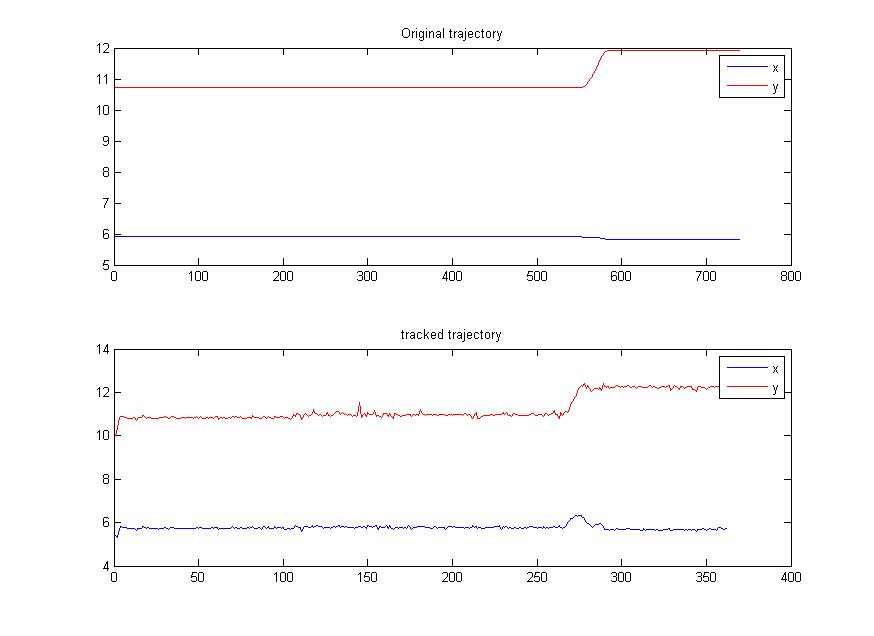
\includegraphics[width=0.5\linewidth]{../Images/c4/arch_trajs}
		\caption{Ejecuci\'on en Odroid - Trayectorias}
		\label{fig:arch_trajs}
	\end{figure}

	
	\subsubsection{Algoritmo de seguimiento est\'ereo}
		En este caso existen dos proveedores de informaci\'on (Dos quadrotors con dos Odroids) que se comunican con la estaci\'on en tierra para el seguimiento del objetivo. La siguiente tabla muestra los tiempos de proceso dentro de la Odroid.
		% 666 TODO: quitar el filtro de media del tratamiento que ralentiza mucho
		\newline
		\newline
		{
		\centering
			\begin{tabular}{|c|c|c|c|c|c|}
			\hline  					&  Open Img	&  cp Img 	& Vicon 	& Treat img & Comm  		\\ 
			\hline  \textbf{time (ms)}	& 	0.0161	& 0.0019	&	0.000098&  	 0.02	&	0.0001		\\ 
			\hline  \textbf{fps (1/s)}	&  	62.11	&  52.631	& 10204.08 	&  49.56	&	986.1	\\ 
			\hline 
			\end{tabular} 
		}
		\newline
		
		Esta segunda tabla muestra los tiempos en la estaci\'on en tierra.
		\newline
		
		{
		\centering
			\begin{tabular}{|c|c|c|}
			\hline  					&  comm		&  EKF step	\\
			\hline  \textbf{time (ms)}	& 	0.0001	& 	0.0001	\\
			\hline  \textbf{fps (1/s)}	&  	10368.5	&   9898.6 	\\
			\hline 
			\end{tabular} 
		}
		\newline
	\begin{figure}[ph]
		\centering
		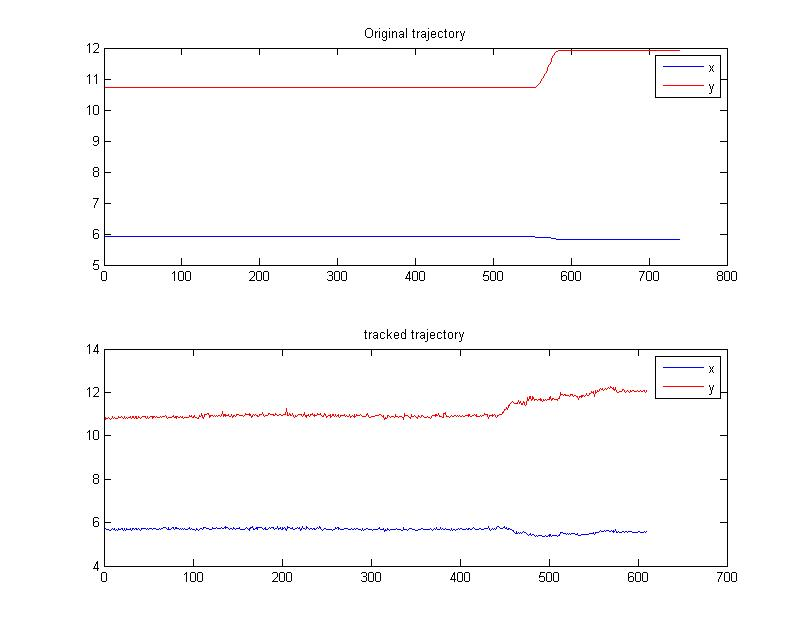
\includegraphics[width=0.7\linewidth]{../Images/c4/arch_trajs_stero}
		\caption{Ejecuci\'on en Odroid - Trayectorias}
		\label{fig:arch_trajs_stero}
	\end{figure}
	
	\begin{figure}[ph]
		\centering
		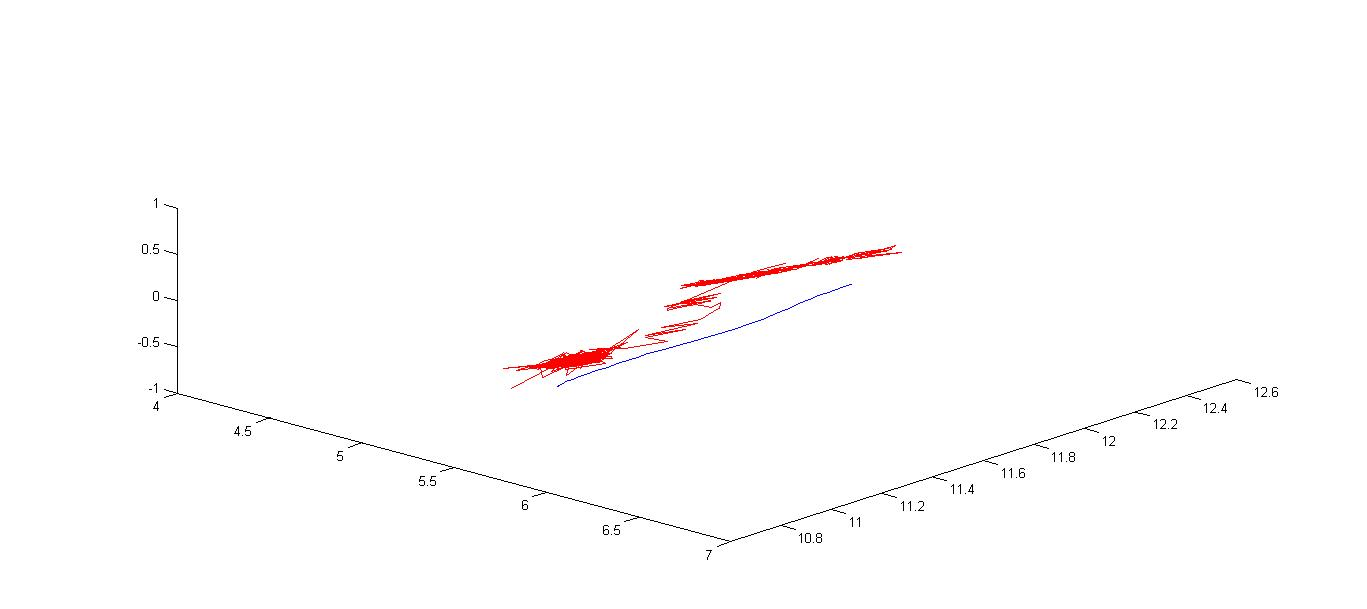
\includegraphics[width=0.6\linewidth]{../Images/c4/arch_3d_trajs_stero}
		\caption{Ejecuci\'on en Odroid - Trayectorias 3D}
		\label{fig:arch_3d_trajs_stero}
	\end{figure}
